\documentclass{article}
\title{テクニカル分析入門 — 数理から見るチャート}
\author{TeX 図書館}

\begin{document}

\section{この教科書のために — チャートを数理で読む}

テクニカル分析は「価格の過去の形から未来を読む」手法の総称です。巷では魔法のように語られたり「全部インチキ」と切り捨てられたりします。この教科書では、主要な手法を\textbf{数理(信号処理・統計)の視点}から理解し、\textbf{何に効いて何に効かないか}を批判的に整理します。

\begin{quote}
\textbf{【心構え】}\ この教科書は特定の売買戦略を推奨しません。『投資の数学』の期待値・資金管理と併読し、「手法の数理的性質」と「実効性の根拠」を分けて考えることが目的です。
\end{quote}

\section{トレンドとノイズ — 信号処理の見方}

価格の動きを\textbf{トレンド成分 + ノイズ成分}の重ね合わせと考えると、テクニカル指標の多くが「ノイズを除去してトレンドを見る道具」(\textbf{フィルタ})であることが分かります。

\begin{quote}
\textbf{【トレードオフの普遍則】}\ フィルタは\textbf{平滑化と遅れ}のトレードオフを必ず持ちます。強く平滑化するほどノイズが消えるが、転換点の検出は遅れる。軽いフィルタは早く反応するがダマシが増える。このトレードオフは物理の測定器と同じで、\textbf{両方得る設定は存在しない}。
\end{quote}

\begin{quote}
\textbf{【演習】}\ 「5 日移動平均」と「200 日移動平均」のうち、ノイズが少ないのはどちらか、遅れが小さいのはどちらか。それぞれの使い所を 1 行で述べよ。
\end{quote}

\textbf{解答の指針:}\ 200 日 = ノイズ少・遅れ大(長期トレンドの確認)。5 日 = 反応早・ダマシ多(短期の局所的な勢い)。

\section{移動平均 — 最も基本的なフィルタ}

\textbf{単純移動平均}( SMA )は直近 \(N\) 日の平均:
\[ \mathrm{SMA}_t(N) = \frac{1}{N}\sum_{i=0}^{N-1} P_{t-i} \]

\begin{figure}[h]
\centering
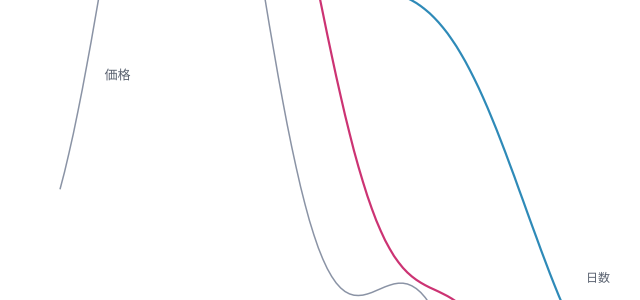
\includegraphics[width=0.85\textwidth]{figures/ma.svg}
\caption{価格と 2 本の移動平均。長期の移動平均ほど滑らかで遅れて動く。}
\end{figure}

改良版として\textbf{指数平滑移動平均}( EMA )があり、新しい価格に重みを多く置きます:
\[ \mathrm{EMA}_t = \alpha P_t + (1 - \alpha)\,\mathrm{EMA}_{t-1} \]
\(\alpha\) が大きいほど反応が速い。SMA が「窓内の全データを等分」なのに対し、EMA は\textbf{指数的に減衰する重み}で過去すべてを永遠に覚えています。

\begin{quote}
\textbf{【演習】}\ EMA で \(\alpha = 0.2\) のとき、5 日前の価格の重みを計算せよ。
\end{quote}

\textbf{解答の指針:}\ 5 日前の重みは \(\alpha(1-\alpha)^4 = 0.2 \times 0.8^4 \approx 0.082\)。減衰は急速で、2 週間前の価格はほとんど影響しない。

\section{ゴールデンクロスとダマシ}

\textbf{ゴールデンクロス}(短期線が長期線を下から上に抜ける)は上昇転換の兆候、\textbf{デッドクロス}はその逆とされます。数理的には\textbf{2 つのフィルタ出力の交差}であり、「短期的な勢いが長期的な水準を上回った」という事実を示します。

ただし\textbf{レンジ相場}(方向のない横ばい)では短期線と長期線が何度も交差し、ダマシが連発します。フィルタの性質として:\textbf{トレンドがある局面ではクロスは有効に働き、トレンドがない局面では機能しない}。トレンドの有無を先に判断するフィルタ(たとえば長期線の傾き)を併用するのはこのためです。

\begin{quote}
\textbf{【演習】}\ 「1 か月で 6 回クロスした」チャートについて、この相場の状態と、クロス戦略の期待値について考察せよ。
\end{quote}

\textbf{解答の指針:}\ レンジ相場。クロスのたびに手数料・スリッページを払うため、期待値はほぼ確実にマイナス。クロス戦略は\textbf{トレンド相場専用の道具}と心得る。

\section{オシレーター — 買われすぎ・売られすぎ}

\subsection{RSI}

\textbf{相対力指数}( RSI )は直近 \(N\) 日の上昇分と下落分の比率:
\[ \mathrm{RSI} = 100 \times \frac{U}{U + D} \]
(\(U\) は上昇幅の平均、\(D\) は下落幅の平均)。0〜100 をとり、慣行では 70 以上で「買われすぎ」、30 以下で「売られすぎ」と見ます。

\subsection{ストキャスティクス}

「現在値が直近レンジのどこに位置するか」の指標。どちらも\textbf{レンジ相場で意味をもつ}指標です——トレンドが続く相場では「買われすぎ」が何週間も続き続けることがあります(RSI の著名な失敗パターン)。

\begin{quote}
\textbf{【演習】}\ 「強い上昇トレンドで RSI が 80 を超えて 3 週間維持」されている局面について、RSI の「買われすぎ = 売り」シグナルが危険な理由を説明せよ。
\end{quote}

\textbf{解答の指針:}\ トレンド相場では上昇日数が連続するため RSI は高止まりするのが\textbf{自然}であり、正規化された値が極端でも転換を意味しない。オシレーターはレンジ用、トレンド判断は移動平均系——道具の対応関係を間違えないこと。

\section{出来高とボラティリティ}

\begin{itemize}
\item \textbf{出来高}: 値動きの\textbf{参加者数}。価格変化に出来高が伴わない場合、その動きは薄手(少数の注文)であり続かないことが多い
\item \textbf{ボラティリティ}: 変動の大きさ。ATR(平均真のレンジ)は 1 日あたりの変動幅の目安で、\textbf{損切り幅やポジションサイズの設計}(『投資の数学』第 7 節)に直接使える
\end{itemize}

\begin{quote}
\textbf{【演習】}\ ATR(14)が 5 円の銘柄に、1 回のリスクを資金の 1\% で取る場合の買い数量の設計手順を述べよ(資金 100 万円)。
\end{quote}

\textbf{解答の指針:}\ 許容損失 = 1 万円。ストップを ATR の 2 倍(10 円)下に置くなら、数量 = 10000/10 = 1000 株。\textbf{損切り幅と数量が連動する}のが規模管理の基本式。

\section{テクニカル分析の限界 — 数理からの批判}

誠実に向き合うべき限界を 3 つ挙げます。

\begin{enumerate}
\item \textbf{効率的市場仮説との緊張}: 価格が(ほぼ)ランダムウォークなら、過去の形は未来の情報を持たない。過去パターンの優位性は、\textbf{多くの参加者が同じチャートを見て同じように反応する自己実現}としてのみ説明可能
\item \textbf{検証の困難}: 「この手法で過去に儲かった」は\textbf{pハッキング}の温床(『統計の誤用事例集』第 6 話)。パラメータ(期間など)を過去データに最適化すると、未来での成績は必ず劣化する(過学習——『機械学習入門』第 5 節と同型)
\item \textbf{コスト}: 手数料・スリッページ・税金は頻繁な取引の期待値を確実に削る。ボリュームが期待値損失の乗数である事実(『投資の数学』第 9 節)はテクニカル売買で最大の敵
\end{enumerate}

\begin{quote}
\textbf{【演習】}\ 「移動平均期間を 5 日から 50 日まで 1 日刻みで試し、最も成績の良い期間を採用した」バックテストの問題点を 2 つ述べよ。
\end{quote}

\textbf{解答の指針:}\ (1) 過去データへの過適合で、選ばれた期間は偶然の産物である可能性が高い。(2) テスト外のデータ(アウトオブサンプル)での検証がないため汎化性能が未知。実務では期間を分割し、別の期間で検証する。

\section{おわりに — 道具として誠実に使う}

この教科書の整理:\textbf{移動平均・オシレーターはフィルタ}(§2〜4)であり、フィルタには平滑化と遅れのトレードオフがつきものです。トレンド系とレンジ系の道具は\textbf{使う局面が違う}(§4)。出来高と ATR(§5)は判断の質と規模管理に役立つ。そして\textbf{過去の形からの予測には理論上の限界}があり(§6)、手法の価値は「誰もが同じ道具を見ている」市場での自己実現性と、\textbf{規模管理の枠組み}としての使い方にあります。

テクニカル分析を「予言機」でなく「\textbf{リスク管理の視覚化道具}」として使う——それが数理から見た誠実な使い方です。

\begin{quote}
\textbf{【総合演習】}
\begin{enumerate}
\item EMA で \(\alpha = 0.5\) のとき、3 期前の価格の重みを求めよ。
\item RSI が高止まりしてもトレンドが続く理由を、「指標の性質」と「相場の状態」の組合せで説明せよ。
\item テクニカル手法のバックテストで過学習を防ぐ方法を 1 つ挙げよ。
\end{enumerate}
\end{quote}

\textbf{解答の指針:}\ 1. \(\alpha(1-\alpha)^2 = 0.5 \times 0.25 = 0.125\)。2. トレンド相場では「上昇日数が多い」ことが状態の自然な帰結であり、正規化された指標が極端な値を示し続けるのは矛盾でない。3. データを学習用と検証用に分け、検証用で成績を確認する(アウトオブサンプル検証)。

\end{document}
